\section{\Sch{} trees and chains in a poset}

\subsection{Partition of a set}

\begin{defi}
	Let $n\in\N$.
	A \emph{partition} of $\IEM{1}{n}$ is a subset $\{I_j\}_{j\in \IEM{1}{k}}$ of $\IEM{1}{n}$ composed of non-empty disjoint subsets such that $\IEM{1}{n}=\displaystyle\bigcup_{j\in\IEM{1}{k}} I_j$.
	We call each of its element $I_j$ a \emph{block}.
\end{defi}

\begin{defi}\label{defi:connexe}
	Let $S\subseteq U$ be a subset of $\mathbb{N}^*$, we call $S$ to be \emph{connected} with respect to $U$ \ssi{} for all $s<t$ pair of elements of $S$, $U\cap \IEM{s}{t}\subseteq S.$ Then, for each part $S\subseteq U$ can be written as a union of connected parts of $U$, called \emph{connected components} of $S$ with respect to $U$.
\end{defi}

Any partition of a set can be represented as a diagram.
\begin{Eg}\label{Eg:partitions}
	For instance consider the partitions of the following set $I=\IEM{1}{10}$:
	\begin{itemize}
		\item $\alpha_0=\IEM{1}{3}$, $\gamma_0=\IEM{4}{7}$ et $\beta_0=\IEM{7}{10}$.
		\item $\alpha_1=\IEM{1}{5}$, $\gamma_1=\{ 6,9,10 \}$ et $\beta_1=\{ 7,8 \}$.
		\item $\alpha_2=\IEM{1}{5}$, $\gamma_2=\{6,8,10\}$ et $\beta_2=\{ 7,9 \}$.
	\end{itemize}
	
	\begin{figure}[h]
		\centering
		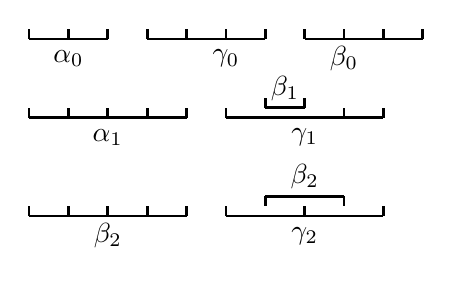
\begin{tikzpicture}[scale=0.5]
			%figure 1
			\draw[line width=1] (0,0) -- (0,0.25);
			\draw[line width=1] (1,0) -- (1,0.25);
			\draw[line width=1] (2,0) -- (2,0.25);
			\draw[line width =1](0,0) -- (2,0);	
			\draw (1,-0.5) node{$\alpha_0$};
			\begin{scope}[shift={(3,0)}]
				\draw[line width=1] (0,0) -- (0,0.25);
				\draw[line width=1] (1,0) -- (1,0.25);
				\draw[line width=1] (2,0) -- (2,0.25);
				\draw[line width=1] (3,0) -- (3,0.25);
				\draw[line width =1](0,0) -- (3,0);	
				\draw (2,-0.5) node{$\gamma_0$}	;
			\end{scope}
			\begin{scope}[shift={(7,0)}]
				\draw[line width=1] (0,0) -- (0,0.25);
				\draw[line width=1] (1,0) -- (1,0.25);
				\draw[line width=1] (2,0) -- (2,0.25);
				\draw[line width=1] (3,0) -- (3,0.25);
				\draw[line width =1](0,0) -- (3,0);	
				\draw (1,-0.5) node{$\beta_0$}	;
			\end{scope}
			%figure 2
			
			\begin{scope}[shift={(0,-2)}]
				\draw[line width=1] (0,0) -- (0,0.25);
				\draw[line width=1] (1,0) -- (1,0.25);
				\draw[line width=1] (2,0) -- (2,0.25);
				\draw[line width=1] (3,0) -- (3,0.25);
				\draw[line width=1] (4,0) -- (4,0.25);
				\draw[line width =1](0,0) -- (4,0);	
				\draw (2,-0.5) node{$\alpha_1$};
			\end{scope}
			
			\begin{scope}[shift={(5,-2)}]
				\draw[line width=1] (0,0) -- (0,0.25);
				\draw[line width=1] (3,0) -- (3,0.25);
				\draw[line width=1] (4,0) -- (4,0.25);
				\draw[line width =1](0,0) -- (4,0);
				\draw (2,-0.5) node{$\gamma_1$};
			\end{scope}	
			
			\begin{scope}[shift={(6,-1.75)}]
				\draw[line width=1] (0,0) -- (0,0.25);
				\draw[line width=1] (1,0) -- (1,0.25);
				\draw[line width =1](0,0) -- (1,0);
				\draw (0.5,0.5) node{$\beta_1$};
			\end{scope}
			
			%figure 3
			\begin{scope}[shift={(0,-4.5)}]
				\draw[line width=1] (0,0) -- (0,0.25);
				\draw[line width=1] (1,0) -- (1,0.25);
				\draw[line width=1] (2,0) -- (2,0.25);
				\draw[line width=1] (3,0) -- (3,0.25);
				\draw[line width=1] (4,0) -- (4,0.25);
				\draw[line width =1](0,0) -- (4,0);	
				\draw (2,-0.5) node{$\beta_2$};
			\end{scope}
			
			\begin{scope}[shift={(5,-4.5)}]
				\draw[line width=1] (0,0) -- (0,0.25);
				\draw[line width=1] (2,0) -- (2,0.25);
				\draw[line width=1] (4,0) -- (4,0.25);
				\draw[line width =1](0,0) -- (4,0);
				\draw (2,-0.5) node{$\gamma_2$};
			\end{scope}	
			
			\begin{scope}[shift={(6,-4)}]
				\draw[line width=1] (0,0) -- (0,-0.25);
				\draw[line width=1] (2,0) -- (2,-0.25);
				\draw[line width =1](0,0) -- (2,0);
				\draw (1,0.5) node{$\beta_2$};
			\end{scope}
		\end{tikzpicture}
	\caption{Some diagrams representing those partitions}
	\end{figure}
\end{Eg}

\begin{defi}
	A partition $\pi$ of \IE{1}{n} is called \emph{non-crossing} if it fulfils the following property :
	\[
	\forall (\gamma_1,\gamma_2)\in \pi^2, \left[\left((i,l)\in\gamma_1^2 \land (j,m)\in \gamma_2^2 \land i\leq j\leq l \leq m \right) \implies \gamma_1=\gamma_2 \right].
	\]
\end{defi}
Taking back the example~\ref{Eg:partitions}, the first and second one are non-crossing partitions but not the last one. 
\begin{Not}
	We will denote $\mathcal{NC}_n$ the set of non-crossing partitions of $\IEM{1}{n}$.
\end{Not}

\begin{defi}
	A partition $\pi$ of \IE{1}{n} is called \emph{monotonous} if it is a non-crossing partition and owes a total order  $\lambda$ over its blocks $\pi$ such that:
	\begin{equation}\label{eq:monotone}
		V \text{ is nested in } W \implies W<_{\lambda} V.
	\end{equation}
	So, we can number those blocks $\pi=\{ V_1,V_2,\cdots, V_l\}$ as $V_1\cup V_2\cup \cdots \cup V_l=\IEM{1}{n}$ such that for all $i,j\in\IEM{1}{l}$, we have :
	\[
	(V_i<_{\lambda} V_j) \iff i<j.
	\]
\end{defi}

\begin{defi}
	Let $n\in\Nz$.
	A partition $\pi$ of \IE{1}{n} is called \emph{interval} if it only has blocks which are their own connected components defined at~\ref{defi:connexe}. 
	We denote by $\IP{n}$ the set of intervals partitions.
\end{defi}

In the previous example~\eqref{Eg:partitions}, only the first one is an interval partition.

\subsection{The poset of interval partitions}

\begin{Not}
	Let $(P\leq)$ be a poset. We denote $<$ the binary relation of $P$ defined for any couple $(x,y)\in P^2$ by:
	\[
	x<y\iff x\leq y \text{ and }x\neq y.
	\]
\end{Not}

\begin{defi}
	Let $n\in\Nz$.
	We define an order over the set $\IP{n}$, given for any $I,J\in\IP{n}$ by:
	\[
	J\leq I \iff \forall J_j\in I, \exists I_i\in J, J_i\subseteq I_j.
	\]
	In other words, $J$ is smaller than $I$ if $J$ is \emph{thinner} than $I$.
	For any $(I,J)\in\IP{n}$ such that $I\leq J$, we say it is a \emph{covering relation} if $I\neq J$ and there does not exist $K\in\IP{n}$ such that $I< K< J.$ 
\end{defi}

\begin{defi}[Chain of a poset]
	Let $(P,\leq)$ be a poset. A \emph{chain} in $P$ is a sequence of elements of $P$ denoted $c=(c_1,\dots,c_k)$ where for all $i\in\IEM{1}{k-1}, c_i<c_{i+1}.$
	A chain $c=(c_1,\dots,c_k)$ is called \emph{maximal}, if for every $i\in\IEM{1}{k-1}$, there does not exist any element $x\in P$ such that $c_1< x<c_k$.
	We call $k$ the \emph{length} of the chain $c$. A \emph{$k$-chain} is a chain of length $k\in\N^*$.
	
	Suppose that $(P,\leq)$ has a minimum and a maximum element respectively denoted $\min(P)$ and $\max(P)$.
	We call an \emph{initial chain} every chain beginning with $\min(P)$ and ending with $\max(P).$ 
	We denote $\C{P}$ the set of initial chains of the poset $P$.
\end{defi}

We can represent a poset as a graph where the edges represent covering relations of the poset.
\begin{Eg}
	For instance, let us draw the poset $\IP{4}$ at figure~\ref{fig:IP4}:
	\begin{figure}[h]
		\centering
		\caption{The \IP{4} poset}
		\label{fig:IP4}
		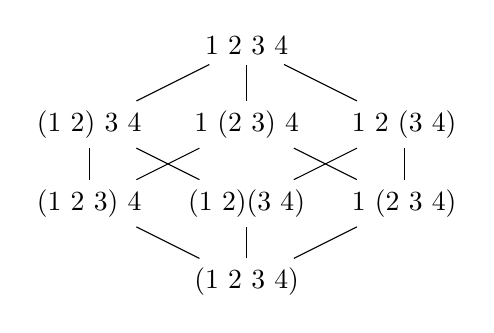
\begin{tikzpicture}
			%Noeud du diagramme
			\node (P0) at (0,0) {$(1~2~3~4)$};
			\node (P11) at (-2,1) {$(1~2~3)~4$};
			\node (P12) at (0,1) {$(1~2)(3~4)$};
			\node (P13) at (2,1) {$1~(2~3~4)$};
			\node(P21) at (-2,2) {$(1~2)~3~4$};
			\node(P22) at (0,2) {$1~(2~3)~4$};
			\node(P23) at (2,2) {$1~2~(3~4)$};
			\node(P31) at (0,3) {$1~2~3~4$};
			%Arêtes du poset
			\draw (P0)--(P11);
			\draw (P0)--(P12);
			\draw (P0)--(P13);
			\draw (P11)--(P21);
			\draw (P11)--(P22);
			\draw (P12)--(P21);
			\draw (P12)--(P23);
			\draw (P13)--(P22);
			\draw (P13)--(P23);
			\draw (P21)--(P31);
			\draw (P22)--(P31);
			\draw (P23)--(P31);
		\end{tikzpicture}
	\end{figure}
\end{Eg}
\begin{defi}[composition of chains in the poset \IP{}]\label{defi:products of chains}
	Let $n,m\in\Nz$ and consider $c$ a $k$-chain of $\IP{n}$ and $d$ a $l$-chain of $\IP{m}$.
	We define many compositions of the two chains $c$ and $d$ as the chain of $\IP{n+m}$ defined by:
	\begin{align*}
		c\circ d&=\left( c_1\cdot d_1,c_2\cdot d_1,\dots, c_k\cdot d_1,c_k\cdot d_2,\dots,c_k\cdot d_l, \IEM{1}{n+m}\right), \\
		c\bullet d&=\left( c_1\cdot d_1,c_1\cdot d_2,\dots, c_1\cdot d_l,c_2\cdot d_l,\dots,c_k\cdot d_l, \IEM{1}{n+m}\right), \\
		c\star d&=\left( c_1\cdot d_1,c_2\cdot d_2,\dots, c_{\min(k,l)}\cdot d_{\min(k,l)}, \dots,c_k\cdot d_l \right),
	\end{align*}
	where $\cdot$ is the concatenation production of partitions shifting the second one by the maximum of the first one.
\end{defi}
%\begin{Rq}
%	Note that $\C{\IP{}}$ is closed for $\circ$.
%\end{Rq}
%Avec cette définition c'est faire priviliégié les opérations à gauche, ceci s'associe à un nivellement de l'arbre canonique de gauche à droite. Il suffit de changer la définition du produit pour avoir une autre forme normale.

\subsection{\Sch{} trees and comb representations}

Let us remind the following definition:
\begin{defi}
	A \emph{\Sch{} tree} is a rooted tree such that any vertices which is not a leaf has at least $2$ children.
	This set can be graded with the number of leaves minus $1$. For any $n\in\Nz$, we define $\Tree_n$ the set of \Sch{} trees with $n+1$ leaves.
\end{defi}
\begin{Not}
	If $t\in\Tree_n$, we define $n\coloneqq \deg(n)$. We will also denote $c_n$ the corolla of degree $n$.
\end{Not}
\begin{Rq}
	As every node of these trees which is not a leaf has at least $2$ children, we will not draw the nodes of a tree any more.
\end{Rq}
\begin{Eg}
	For instance, here is some examples of \Sch{} trees:
	\[
	\Y,\balaisg, \balaisd,\balais, \YY.
	\]
\end{Eg}

Let $t$ be a tree. It $t$ can always be seen as:
\begin{center}
	\raisebox{-0.5\height}{\begin{tikzpicture}[line cap=round,line join=round,>=triangle 45,x=0.5cm,y=0.5cm]
			% Etage 1
			\draw (0,0)--(0,1);
			%Etage 2
			\draw (0,1)--(-2,2) node[above]{$t^1_1$};
			\draw (0,1)--(0,2) node[above]{$t^1_{n_1}$};
			\draw (-1,2) node{$\cdots$};
			% Etage 3
			\draw (0,1)--(7,8);
			\draw (3,4)--(1,5) node[above]{$t^2_1$};
			\draw (3,4)--(3,5) node[above]{$t^2_{n_2}$};
			\draw (2,5) node{$\cdots$};
			%Etage...
			\draw (4.7,6) node[rotate=45]{$\cdots$};
			%Etage k
			\draw (6,7)--(4,8) node[above]{$t^k_1$};
			\draw (6,7)--(6,8) node[above]{$t^k_{n_k}$};
			\draw (5,8) node {$\cdots$};
	\end{tikzpicture}},
\end{center}
where $k$ is the number of nodes on the right-most branch of $t$ and for $i\in\IEM{1}{k}, n_i+1$ is the number of sons of the $i$-th node of this branch.

\begin{Not}
	Let $F=t_1\dots t_n$ be a forest composed of $n$ trees. Instead of writing:
	\begin{center}
		\raisebox{-0.5\height}{\begin{tikzpicture}[line cap=round,line join=round,>=triangle 45,x=0.5cm,y=0.5cm]
				% Etage 1
				\draw (0,0)--(0,1);
				%Etage 2
				\draw (0,1)--(-2,2) node[left,above]{$t_1$};
				\draw (0,1)--(0,2) node[right,above]{$t_{n}$};
				\draw (-1,2) node{$\cdots$};
				\draw (0,1)--(2,2);
		\end{tikzpicture}},
	\end{center}
	we will write:
	\raisebox{-0.3\height}{\begin{tikzpicture}[line cap=round,line join=round,>=triangle 45,x=0.3cm,y=0.3cm]
			% Etage 1
			\draw (0,0)--(0,1);
			%Etage 2
			\draw (0,1)--(-1,2) node[left]{$F$};
			\draw (0,1)--(1,2);
	\end{tikzpicture}}.
\end{Not}

As a consequence, we deduce that all tree $t$ can be seen as:
\begin{center}
	\raisebox{-0.5\height}{\begin{tikzpicture}[line cap=round,line join=round,>=triangle 45,x=0.3cm,y=0.3cm]
			% Etage 1
			\draw (0,0)--(0,1);
			%Etage 2
			\draw (0,1)--(-1,2) node[left]{$F_1$};
			% Etage 3
			\draw (0,1)--(6,7);
			\draw (2,3)--(1,4) node[left]{$F_2$};
			%Etage...
			\draw (3.,4.5) node[rotate=45]{$\cdots$};
			%Etage k
			\draw (5,6)--(4,7) node[left]{$F_k$};
	\end{tikzpicture}},
\end{center}
where $F_1,\dots,F_k$ are non-empty forests.
\begin{defi}
	The writing defined above is the writing of $t$ as a \emph{right comb}.
	Proceeding the same way, looking at the left branch of the root of $t$, we get the writing of $t$ as a \emph{left comb}.
\end{defi}


\subsection{Our objective}

\begin{defi}\label{def:tridend}
	Let $\K$ be a field and $A$ be vector space of $\K$. We say $(A,\prec,\cdot,\succ)$ is a \emph{tridendriform algebra} if $\prec,\cdot$ and $\succ$ are all linear maps from $A\otimes A$ to $A$ such that for any $a,b,c\in A$:
	\begin{align}
		(a\prec b)\prec c&=a\prec(b*c), \label{eq:tri1}\\
		(a\succ b)\prec c&=a\succ(b\prec c), \label{eq:tri2} \\
		(a* b)\succ c&=a\succ(b\succ c),  \label{eq:tri3} \\
		(a\succ b)\cdot c&=a\succ(b\cdot c), \label{eq:tri4} \\
		(a\prec b)\cdot c&=a\cdot(b\succ c), \label{eq:tri5} \\
		(a\cdot b)\prec c&=a\cdot(b\prec c), \label{eq:tri6} \\
		(a\cdot b)\cdot c&=a\cdot (b\cdot c), \label{eq:tri7}
	\end{align}
	where $*$ is the \emph{associative product} of the tridendriform algebra defined for any $a,b\in A$ by $a*b\coloneqq a\prec b + a\cdot b +a\succ b$. 
	We call the products $\succ,\prec,\cdot$ respectively right, left and middle.
\end{defi} 

The free tridendriform algebra is built on the vector space $\K\Tree \oplus \K\cdot |$ where $|$ is the unit of the product $*$. We will denote it by $(\A,\prec,\cdot,\succ)$. We have a combinatorial interpretation of the product $*$. For this let us introduce:
\begin{defi}[Quasi-shuffle]
	Let $k,l\in\N\setminus \{0\}$. A \emph{$(k,l)$-quasi-shuffle} is a surjective map $\sigma:\IEM{1}{k+l}\twoheadrightarrow\IEM{1}{n}$ surjective for some positive integer $n$
	such that:
	\[
	\sigma(1)<\cdots<\sigma(k) \text{  and  } \sigma(k+1)<\cdots<\sigma(k+l).
	\]
	We will denote $\batc(k,l)$ the set of all $(k,l)$-quasi-shuffles.
\end{defi}
 
 
 Let $t,s$ two trees different from $|$. We look $t$ as a right comb and $s$ as a left comb. In other words, we put:
 \begin{align*}
 	t&=\peignedroit{1}{2}{k}
 	& \text{ and } &&  s=\peignegauche{k+1}{k+2}{k+l},
 \end{align*}
 where for all $i\in\IEM{1}{k+l}, F_i$ is a non-empty forest. Here, $k$ represents the number of nodes on the right-most branch of $t$ and $l$ is the number of nodes on the left-most branch of $s$.
 
 \begin{defi}\label{def:quasiaction}
 	Let $t$ and $s$ be two trees which respective right comb representation and left comb representation are given above.
 	We denote by $k$ (respectively $l$) the number of nodes on the right-most (respectively left-most) branch of $t$ (respectively $s$). Let $\sigma$ be a $(k,l)$-quasi-shuffle which has for image $\IEM{1}{n}$ for $n$ a positive integer. We denote $\sigma(t,s)$ the tree obtained this way:
 	\begin{enumerate}
 		\item  We first consider the ladder with $n$ nodes:
 		\begin{center}
 			\raisebox{-0.5\height}{\begin{tikzpicture}[line cap=round,line join=round,>=triangle 45,x=0.3cm,y=0.3cm]
 					\begin{scope}{shift={(-3,0)}}
 						\draw (0,0)--(0,2.5);
 						\draw[dashed] (0,2.5)--(0,5);
 						\draw (0,5)--(0,6);
 						\filldraw [black] (0,1) circle (2pt) node[anchor=west]{Node $1$};
 						\filldraw [black] (0,2) circle (2pt) node[anchor=west]{Node $2$};
 						\filldraw [black] (0,5) circle (2pt) node[anchor=west]{Node $n$};
 					\end{scope}
 			\end{tikzpicture}}.
 		\end{center}
 		\item For all $i\in\IEM{1}{k},$ we graft $F_i$ as the \emph{left} son at the node $\sigma(i)$.
 		\item For all $i\in\IEM{k+1}{k+l},$ we graft $F_i$ as \emph{right} son at the node $\sigma(i)$.
 	\end{enumerate}
 \end{defi}
 
 \begin{Eg}\label{Eg:quasiaction}
 	Consider the $(2,2)$-quasi-shuffle $\sigma=(1,3,2,3)$. Let us take:
 	
 	$t=$	\raisebox{-0.3\height}{\begin{tikzpicture}[line cap=round,line join=round,>=triangle 45,x=0.2cm,y=0.2cm]
 			% Etage 1
 			\draw (0,0)--(0,1);
 			%Etage 2
 			\draw (0,1)--(-1,2) node[left]{$F_1$};
 			% Etage 3
 			\draw (0,1)--(2,3);
 			\draw (1,2)--(0,3) node[left,above]{$F_2$};
 	\end{tikzpicture}} and $s=$ \raisebox{-0.3\height}{\begin{tikzpicture}[line cap=round,line join=round,>=triangle 45,x=0.2cm,y=0.2cm]
 			% Etage 1
 			\draw (0,0)--(0,1);
 			%Etage 2
 			\draw (0,1)--(1,2) node[right]{$F_{3}$};
 			% Etage 3
 			\draw (0,1)--(-2,3);
 			\draw (-1,2)--(0,3) node[right,above]{$F_{4}$};
 	\end{tikzpicture}}.
 	Then $\sigma(t,s)=$\raisebox{-0.5\height}{\begin{tikzpicture}[line cap=round,line join=round,>=triangle 45,x=0.3cm,y=0.3cm]
 			\draw (0,0)--(0,4);
 			%Noeud 1
 			\draw (0,1)--(-1,2) node[left]{$F_1$};
 			%Noeud 2
 			\draw (0,2)--(1,3) node[right]{$F_3$};
 			%			%Noeud 3
 			\draw (0,3)--(-1,4) node[left]{$F_2$};
 			\draw (0,3)--(1,4) node[right]{$F_4$};
 	\end{tikzpicture}}.
 \end{Eg} 
 
 \begin{thm}\label{thm:produit}
 	Let $t,s$ be two trees different from $|$ as described above. Then: 
 	\[
 	t*s=\sum_{\sigma\in \batc(k,l)}\sigma(t,s).
 	\]
 	Moreover:
 		\begin{align*}
 		t\prec s&=\sum_{\substack{\sigma\in\batc(k,l) \\ \sigma^{-1}(\{1\})=\{1\}}} \sigma(t,s), \\
 		t\cdot s&=\sum_{\substack{\sigma\in\batc(k,l) \\ \sigma^{-1}(\{1\})=\{1,k+1\}}} \sigma(t,s), \\
 		t\succ s&=\sum_{\substack{\sigma\in\batc(k,l) \\ \sigma^{-1}(\{1\})=\{k+1\}}} \sigma(t,s).
 	\end{align*}
 \end{thm}
 Surprisingly,  $(\A,\prec,\cdot,\succ)$ can be endowed with a codendriform coproduct given by:
 
 \begin{thm}\label{thm:coproduit}
 	We define the map over $\mathcal{A}$ for all trees $t$ by the formula:
 	\begin{align*}
 		\Delta(t)&=\sum_{c \text{ \normalfont admissible cut of }t} G^c(t)\otimes R^c(t), \\
 		\Delta(|)&=|\otimes |,
 	\end{align*}
 	where $R^c(t)$ is the component of $t$ containing its root and $G^c(t)=G^c_1(t)*\cdots *G^c_k(t)$, where $G^c_i(t)$ are naturally ordered from left to right. More over one can define:
 	\begin{align*}
 		\Delta_{\leftarrow}(t)&=\sum_{\substack{c \text{ \normalfont admissible cut of }t \\ \text{ \normalfont the right-most leaf of $t$ is cut}}} G^c(t)\otimes R^c(t), \\
 		\Delta_{\rightarrow}(t)&=\sum_{\substack{c \text{ \normalfont admissible cut of }t \\ \text{ \normalfont the right-most leaf of $t$ is not cut}}} G^c(t)\otimes R^c(t).
 	\end{align*}
 Hence, $(\A,\prec,\cdot,\succ,\Delta_{\leftarrow},\Delta_{\rightarrow})$ is a $(3,2)$-dendriform bialgebra.
 \end{thm}

Hence, a natural question is to compute the primitives of $\A$. Let us introduce the notations to reach the theorems for this purpose:
\begin{defi}
	Let $(C,\Delta_{\leftarrow},\Delta_{\rightarrow})$ be a dendriform coalgebra. We define:
	\begin{align*}
		\Prim_{\leftarrow}(C)&:=\{ c\in C \,|\, \tilde{\Delta}_{\leftarrow}(c)=0 \}, \\
		\Prim_{\rightarrow}(C)&:=\{ c\in C \,|\, \tilde{\Delta}_{\rightarrow}(c)=0 \}, \\
		\Prim_{\Coass}(C)&:=\{ c\in C \,|\, \tilde{\Delta}(c)=0 \},\\
		\Prim_{\Codend}(C)&:=\{ c\in C \,|\, \tilde{\Delta}_{\leftarrow}(c)=\tilde{\Delta}_{\rightarrow}(c)=0 \}.
	\end{align*}
\end{defi}

\begin{thm}\label{thm:coassincodend}
	For all $n\in\N$, we define:
	\begin{equation*}
		\theta_n:\left\lbrace \begin{array}{rcl}
			\Prim_{\Coass}(\mathcal{A})_n& \rightarrow & \Prim_{\Codend}(\mathcal{A})_{n+1} \\
			a\otimes \Y & \mapsto & a\cdot \Y.
		\end{array}\right.
	\end{equation*}
	Then, for all $n\in\N, \theta_n$ is an isomorphism of vector spaces.
\end{thm}

From the article~\cite{euleridem} of M.\bsc{Ronco}, we recall the global construction:
\begin{defi}[brace algebra]
	A \emph{brace algebra} is a $\K$-vector space $B$ endowed for any $n\in\N$ of linear maps:
	\[
	M_n:\left\lbrace\begin{array}{rcl}
		B^{\otimes n} & \rightarrow & B, \\
		b_1\otimes\dots\otimes b_n& \mapsto & M_n(b_1\otimes\dots\otimes b_n),
	\end{array} \right.
	\] with $M_1=\Id_V$ such that for all $m,n\in\N\setminus\{0\}, a_1,\dots,a_m,b_1,\dots,b_n,c\in B$:
	\begin{align*}
		&M_{m+1}(a_1\otimes\dots\otimes a_m\otimes M_{n+1}(b_1\otimes\dots\otimes b_n\otimes c)) \\
		=&\sum_{\boldsymbol{A}} M\left(A_0\otimes M(A_1\otimes b_1)\otimes A_2\otimes M(A_3\otimes b_2)\otimes A_4\otimes\dots\otimes A_{2n-2}\otimes M(A_{2n-1}\otimes b_n)\otimes A_{2n}\otimes c\right),
	\end{align*}
	where $\boldsymbol{A}$ is a of the tensor $a_1\otimes \dots \otimes a_m$ i.e $\boldsymbol{A}=(A_0,\dots,A_{2n})\in T(B)^{2n}$ such that:
	\[
	a_1\otimes \dots \otimes a_m=A_0\otimes A_1\otimes \dots\otimes A_{2n-1}\otimes A_{2n}.
	\]
\end{defi}
\begin{Eg}
	One example of such a relation is:
	\[
	M_2(a,M_2(b,c))=M_3(a,b,c)+M_3(b,a,c)+M_2(M_2(a,b),c).
	\]
\end{Eg}
\begin{Not}
	We will denote the free brace algebra generated by a set $X$ by $\Br(X).$
\end{Not}
\begin{defi}
	We define the following operators in $\A$:
	\[
	\omega_{\prec}:\left\lbrace\begin{array}{rcl}
		T(D)^+ & \rightarrow & D, \\
		x_1\otimes \dots\otimes x_n &\mapsto &\begin{cases}
			x_1 & \text{ if }n=1,\\
			\omega_{\prec}(x_1\otimes\dots\otimes x_{n-1})\prec x_n &\text{ else.} 
		\end{cases} 
	\end{array} \right.
	\]
	For all $n\in\N$, we introduce the map $\omega:\bigcup_{n\in\N^*} D^n \rightarrow D$ defined for all ${x_1,\dots, x_n\in D}, {y\in D}$ by:
	\begin{align*}
		\omega(y)&=y,\\
		\omega(x_1\otimes \dots\otimes x_n\otimes y)&\coloneqq \sum_{i=0}^n (-1)^{n-i} \omega_{\prec}(x_1\otimes \dots\otimes x_i)\succ y\prec \omega_{\succ}(x_{i+1},\dots,x_n).
	\end{align*}
\end{defi}
\begin{Rq}
	This quantity is not ambiguous thanks to relation~$\eqref{eq:tri2}$.
\end{Rq}
\begin{Not}
	For all $n\in\N$, we denote by $\omega_{n-1}=\omega|_{D^{\otimes n}}$.
\end{Not}
Here is one the second fundamental result:
\begin{thm}\label{thm:génération2}
	For all $n\in\N$:
	\begin{equation}\label{eq:Omega}
		\Omega_n:\left\lbrace\begin{array}{rcl}
			T(\Prim_{\Codend}(\A))_n & \twoheadrightarrow & \Prim_{\Coass}(\A)_n, \\
			x_1\otimes\dots\otimes x_k & \mapsto & \omega(x_1\otimes \dots \otimes x_k),
		\end{array}\right.
	\end{equation}
	This raise to a map $\Omega$ defined over $\A$ such that $\Omega|_{T(\Prim_{\Codend}(\A))_n}=\Omega_n$.
\end{thm}

As a consequence, we have a recipee to produce the primitives of this algebra by induction:
\begin{figure}[h]
	\centering
	\begin{tikzcd}
		\left\{\Y\right\}=\Prim_{\Codend}(\A)_1 \arrow[r,"\theta_1"] &\Prim_{\Coass}(\A)_2 \arrow[r,"\Omega_1"] & \Prim_{\Codend}(\A)_2 \arrow[r,"\theta_1"] & \Prim_{\Codend}(\A)_3 \arrow[r,"\Omega_2"]& \dots
	\end{tikzcd}
\caption{Diagram of the induction}
\label{fig:algo_idea}
\end{figure}

This diagram allows us to compute $\Prim_{\Coass}(A)$ by induction over the degree of its elements. We will now look at the practical aspects to implement an algorithm on a computer. 


 \subsection{From \Sch{} trees to chains in the interval partition poset}
 
 \subsubsection{From trees to chains}
 Our first objective is to implement \Sch{} trees in a computer. To complete this objective, we have:
 \begin{Prop}\label{tree=ini_chain}
 	Let $n\in\Nz$ and $\ltimes\in\{\circ,\bullet,\star\}$
 	Then, there exists an injection not surjective:
 	\[
 	\Phi_{\ltimes}:\left\lbrace\begin{array}{rcl}
 		\Tree_n & \rightarrow &\C{\IP{n}}, \\
 		t & \mapsto & \Phi_{\ltimes}(t),
 	\end{array} \right.
 	\]
 	where $\Phi_{\ltimes}(t)$ can be defined by induction as follows:
 	\begin{align*}
 		\Phi_{\ltimes}(c_n)&=(1~2~\dots~n~n+1,\IEM{1}{n+1}), \\
 		\Phi_{\ltimes}\left(\corollagraft{1}{2}{k}{k+1} \right)&=\left(\Phi_{\ltimes}(t_1)\circ\Phi_{\ltimes}(t_2)\circ\dots\circ\Phi_{\ltimes}(t_n)\circ \Phi_{\ltimes}(t_{n+1}),\IEM{1}{n+m}\right).
 	\end{align*}
 \end{Prop}
As a consequence, one can see a tree $t$ as an initial chain in the a poset $\IP{}.$ This map is clearly not surjective as $\left( 1~2~3~4,(1~2)(3~4),\IEM{1}{4}\right)$ cannot be in the image of $\Phi_{\circ}$ and $\Phi_{\bullet}$ and $\left(1~2~3~4,(1~2)~3~4,(1~2)(3~4),\IEM{1}{4} \right)$ is not in the image of $\Phi_{\star}$.
These maps $\Phi$ may seem mysterious, but just compute this on the example:
\begin{Eg}
	Consider the tree $t$ given below:
	\[
	\raisebox{-0.5\height}{\begin{tikzpicture}[line cap=round,line join=round,>=triangle 45,x=0.2cm,y=0.2cm]
			\draw (0,0)--(0,5);
			\draw (0,1)--(-4,5);
			\draw (-2.5,3.5)--(-1,5);
			\draw (-2,4)--(-3,5);
			\draw (0,1)--(4,5);
			\draw (2.5,3.5)--(2.5,5);
			\draw (2.5,3.5)--(1,5);
			\draw (1.5,4.5) -- (2,5);
	\end{tikzpicture}}
	\]
	Then, $\Phi(t)$ is the following initial chain:
	\begin{align*}
		& \Phi_{\circ}(t)= &&	\Phi_{\star}(t)= && \Phi_{\bullet}(t)= \\
		&1~2~3~4~5~6~7~8~9, &&  1~2~3~4~5~6~7~8~9, && 1~2~3~4~5~6~7~8~9, \\ 
		&1~(2~3)~4~5~6~7~8~9, && 1~(2~3)~4~5~(6~7)~8~9, && 1~2~3~4~5~(6~7)~8~9,\\
		&(1~2~3)~4~5~6~7~8~9, && (1~2~3)~4~5~(6~7~8~9), && 1~2~3~4~5~(6~7~8~9),\\
		&(1~2~3~4)~5~6~7~8~9, && (1~2~3~4)~5~(6~7~8~9), &&  1~(2~3)~4~5~(6~7~8~9),\\
		&(1~2~3~4)~5~(6~7)~8~9, && (1~2~3~4)~5~(6~7~8~9), && (1~2~3)~4~5~(6~7~8~9),\\
		&(1~2~3~4)~5~(6~7~8~9), && (1~2~3~4~5~6~7~8~9), && (1~2~3~4)~5~(6~7~8~9),\\
		&(1~2~3~4~5~6~7~8~9). &&						&& (1~2~3~4~5~6~7~8~9).
	\end{align*} 
\end{Eg}
As a consequence, one can see a \Sch{} tree as an initial chain in some $\IP{}$. This will be a way we use to implement \Sch{} trees in a computer.

\subsubsection{From initial chains to trees}

\begin{Not}
	Let $t$ be a tree with labelled leaves in a subset $I\subseteq \Nz$, we put:
	\[
	\Leaf(t)=I.
	\]
\end{Not}

\begin{defi}
	We introduce $T(\Tree)$ the tensor algebra with trees as letters. A \emph{forest} is a word from $T(\Tree).$
\end{defi}

\begin{defi}
	Let $n\in\Nz$.
	Let $F$ be a forest of trees with $n$ leaves indexed by $\IEM{1}{n}$. We map a partition $\pi$ of $\IEM{1}{n}$ from $F=t_1\dots t_k$ as:
	\[
	\pi=\bigcup_{i=1}^k\left\{\Leaf(t_i)\right\}.
	\] 
	We denote $\pi\coloneqq\Par(F)$.
\end{defi}
\begin{Eg}
	Consider the forest $F=\labYY{1}{2}{3}{5}~\labbalais{4}{6}{7}$. Then:
	\[
	\Par(F)=\left\{\{1,2,3,5\},\{4,6,7\}\right\}.
	\]
\end{Eg}
\begin{Rq}
	If we label the leaves of a forest $F$ from left to right, we have $\Par(F)\in\IP{n}$. 
\end{Rq}
\begin{defi}
	Let $n$ and $k$ be two elements of $\Nz$. Consider $\pi=\left\{\pi_1,\dots,\pi_s\right\}$ be an element of $\IP{n}$ and let $F=t_1\dots t_k$ be a forest of $k$ trees with a total of $n$ leaves indexed by $\IEM{1}{n}$ from left to right such that:
	\[
	\pi\leq\Par(F).
	\] 
	We define $\Psi_{\pi}(F)$ the forest defined by:
	\[
	t_1\vee \dots\vee t_{l_1} ~t_{l_1+1}\vee\dots\vee t_{l_2+1}~\dots~t_{l_s}\vee\dots\vee t_{k}
	\]
	where $1\leq l_1\leq\dots\leq t_{l_s}\leq n$ and:
	\[
	\forall s\in\IEM{1}{s}, \bigcup_{i=1}^s \Leaf(t_{i})=\pi_i.
	\] 
\end{defi}
\begin{Eg}
	Consider:
	\[
	F=\labbalais{2}{1}{3}~|^4~\labYY{5}{6}{7}{8}~\labbalaisd{9}{10}{11}.
	\]
	and $\pi=\left\lbrace \IEM{1}{4}, \IEM{5}{11}\right\rbrace$ then:
	\[
	\Psi_{\pi}(F)=\raisebox{-0.4\height}{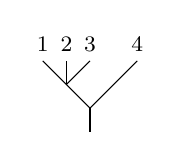
\begin{tikzpicture}[x=0.3cm,y=0.3cm]
		\draw (0,0)--(0,1);
		\draw (0,1)--(-2,3);
		\draw (-1,2)--(-1,3);
		\draw (-1,2)--(0,3);
		\draw (0,1)--(2,3);
		%décorations
		\draw (-2,3) node[above] {\footnotesize{1}};
		\draw (-1,3) node[above] {\footnotesize{2}};
		\draw (0,3) node[above] {\footnotesize{3}};
		\draw (2,3) node[above] {\footnotesize{4}};
	\end{tikzpicture}}
~\raisebox{-0.4\height}{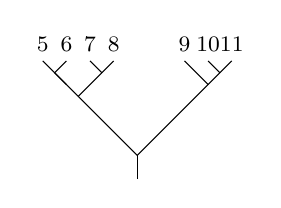
\begin{tikzpicture}[x=0.3cm, y=0.3cm]
	\draw (0,0) -- (0,1);
	\draw (0,1) -- (-4,5);
	\draw (-3.5,4.5) -- (-3,5);
	\draw (-3.5,4.5) -- (-3,4);
	\draw (-2.5,3.5) -- (-1,5);
	\draw (-1.5,4.5) -- (-2,5);
	\draw (0,1) -- (4,5);
	\draw (3.5,4.5) -- (3,5);
	\draw (3,4) -- (2,5);
	%décorations
	\draw (-4,5) node[above] {\footnotesize{5}};
	\draw (-3,5) node[above] {\footnotesize{6}};
	\draw (-2,5) node[above] {\footnotesize{7}};
	\draw (-1,5) node[above] {\footnotesize{8}};
	\draw (2,5) node[above] {\footnotesize{9}};
	\draw (3,5) node[above] {\footnotesize{10}};
	\draw (4,5) node[above] {\footnotesize{11}};
\end{tikzpicture}}.
	\]
\end{Eg}

\begin{defi}
	Let $n,k\in\Nz$.
	Consider $c=(c_1,\dots,c_k)$ be an element of $\IP{n}$. We define $\Psi(c)$ as:
	\[
	\Psi_{c_k}\circ\Psi_{c_{k-1}}\circ \dots\Psi_{c_2}(|^1\dots |^n).
	\]
\end{defi}
\begin{Rq}
	This equation is well defined
\end{Rq}
\begin{Eg}\label{Eg:tree_left}
For instance, consider the chain $c$ given below:
	\begin{align*}
		\left( 1~2~3~4~5~6~7~8~9,  
		1~(2~3)~4~5~(6~7)~8~9, 
		(1~2~3)~4~5~(6~7~8~9),
		(1~2~3~4)~5~(6~7~8~9),
		(1~2~3~4~5~6~7~8~9)\right).
	\end{align*}
	Then, we build $\Psi(c)$ step by step:
\begin{center}
	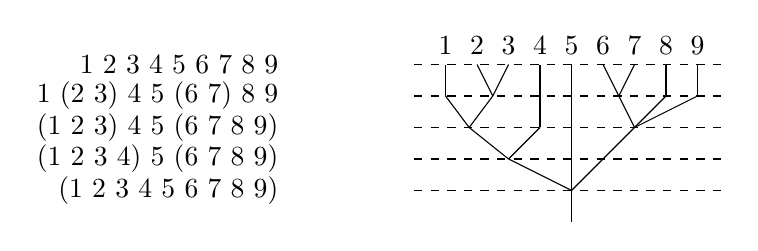
\begin{tikzpicture}[x=0.4cm,y=0.4cm]
		%décorations
		\draw (-4,5) node[above] {$1$};
		\draw (-3,5) node[above] {$2$};
		\draw (-2,5) node[above] {$3$};
		\draw (-1,5) node[above] {$4$};
		\draw (0,5) node[above] {$5$};
		\draw (1,5) node[above] {$6$};
		\draw (2,5) node[above] {$7$};
		\draw (3,5) node[above] {$8$};
		\draw (4,5) node[above] {$9$};
		%Etage 0
		\draw (-4,5) -- (-4,4);
		\draw (-3,5) -- (-2.5,4);
		\draw (-2,5) -- (-2.5,4);
		\draw (-1,5) -- (-1,4);
		\draw (0,5) -- (0,4);
		\draw (1,5) -- (1.5,4);
		\draw (2,5) -- (1.5,4);
		\draw (3,5) -- (3,4);
		\draw (4,5) -- (4,4);
		%Etage -1
		\draw (-4,4) -- (-3.25,3);
		\draw (-2.5,4) -- (-3.25,3);
		\draw (-1,4) -- (-1,3);
		\draw  (0,4) -- (0,3);
		\draw (1.5,4) -- (2,3);
		\draw (3,4) -- (2,3);
		\draw (4,4) -- (2,3);
		%Etage -2
		\draw (-3.25,3)--(-2,2);
		\draw (-1,3) -- (-2,2);
		\draw  (0,3) -- (0,2);
		\draw (2,3) -- (0,1);
		%Etage -3
		\draw (-2,2) -- (0,1);
		\draw (0,2) -- (0,0);
		%Lien avec la chaîne
		\draw[dashed] (-5,5)--(5,5);
		\draw (-9,5) node[left]{$1~2~3~4~5~6~7~8~9$};
		\draw[dashed] (-5,4)--(5,4);
		\draw (-9,4) node[left]{$1~(2~3)~4~5~(6~7)~8~9$};
		\draw[dashed] (-5,3)--(5,3);
		\draw (-9,3) node[left]{$(1~2~3)~4~5~(6~7~8~9)$};
		\draw[dashed] (-5,2)--(5,2);
		\draw (-9,2) node[left]{$(1~2~3~4)~5~(6~7~8~9)$};
		\draw (-9,1) node[left]{$(1~2~3~4~5~6~7~8~9)$};
		\draw[dashed] (-5,1)--(5,1);
	\end{tikzpicture}
\end{center} 
Hence:
\[
\Psi(c)=\raisebox{-0.5\height}{\begin{tikzpicture}[line cap=round,line join=round,>=triangle 45,x=0.2cm,y=0.2cm]
		\draw (0,0)--(0,5);
		\draw (0,1)--(-4,5);
		\draw (-2.5,3.5)--(-1,5);
		\draw (-2,4)--(-3,5);
		\draw (0,1)--(4,5);
		\draw (2.5,3.5)--(2.5,5);
		\draw (2.5,3.5)--(1,5);
		\draw (1.5,4.5) -- (2,5);
\end{tikzpicture}}.
\]
\end{Eg}
So, for all $n\in\Nz$ it gives a map $\Psi:\Tree_n\rightarrow \C{\IP{n}}$. Moreover, for any $\ltimes\in\{\circ,\bullet,\star\}$, we have the commutative diagram:
\begin{figure}
	\centering
		\begin{tikzcd}
			\Tree_n \arrow[r, bend left=45, "\Psi"]& \C{\IP{n}}\arrow[l,bend left=45,"\theta_{\ltimes}"].
		\end{tikzcd} 
	\caption{The map $\Psi$ and some sections}
	\label{fig:Psi}
\end{figure}
In other words, $\theta_{\ltimes}$ is a section of $\Psi.$

\begin{Rq}
	Let $n\in\Nz$:
	\begin{itemize}
		\item if $c\in\C{\IP{n}}$ is a maximal chain then $\Psi(c)$ is a rooted binary tree.
		\item if one considers levelled \Sch{} trees, then there is a bijection between the set $\C{\IP{n}}$ and levelled \Sch{} trees. 
	\end{itemize}
\end{Rq}

As we previously stated, in a computer a tree will be encoded as an element of $\C{\IP{}}$. In order to compute the primitive elements given by the inductive figure~\ref{fig:algo_idea}, one needs to understand the computations of theorem~\ref{thm:produit} with the initial chain point of view.

\section{Correspondence between trees and initial chains of a poset}

One annoying fact about the poset described in figure~\ref{fig:IP4} is that a Schroeder tree may be represented by two different chains in this poset. To solve this problem, we introduce a distorted version of this poset.
For this aim, first consider a labelling of the edges of the poset given in figure~\ref{fig:labelled_IP4}. In this figure, the label $k$ of an edge represents the fusion of block $k$ with the following. 
	\begin{figure}[h]
	\centering
	\caption{The \IP{4} poset with labels on edges}
	\label{fig:labelled_IP4}
	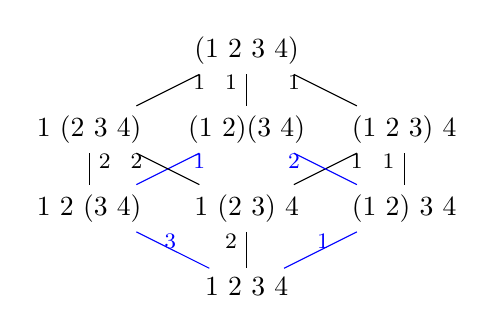
\begin{tikzpicture}[rotate =180 ]
		%Noeud du diagramme
		\node (P0) at (0,0) {$(1~2~3~4)$};
		\node (P11) at (-2,1) {$(1~2~3)~4$};
		\node (P12) at (0,1) {$(1~2)(3~4)$};
		\node (P13) at (2,1) {$1~(2~3~4)$};
		\node(P21) at (-2,2) {$(1~2)~3~4$};
		\node(P22) at (0,2) {$1~(2~3)~4$};
		\node(P23) at (2,2) {$1~2~(3~4)$};
		\node(P31) at (0,3) {$1~2~3~4$};
		%Arêtes du poset
		\draw (P0) -- (P11) node[left,near start] {\footnotesize{$1$}};
		\draw (P0) -- (P12) node[left,near start] {\footnotesize{$1$}};
		\draw (P0) -- (P13) node[right,near start] {\footnotesize{$1$}};
		\draw (P11) -- (P21) node[left,near start] {\footnotesize{$1$}};
		\draw (P11) -- (P22) node[right,near start] {\footnotesize{$1$}};
		\draw[blue] (P12) -- (P21) node[left, near start] {\footnotesize{$2$}};
		\draw[blue] (P12) -- (P23) node[right,near start] {\footnotesize{$1$}};
		\draw (P13) -- (P22) node[left,near start] {\footnotesize{$2$}};
		\draw (P13) -- (P23) node[right,near start] {\footnotesize{$2$}};
		\draw[blue] (P21) -- (P31) node[left,near start] {\footnotesize{$1$}};
		\draw (P22) -- (P31) node[left,near start] {\footnotesize{$2$}};
		\draw[blue] (P23) -- (P31) node[right,near start] {\footnotesize{$3$}};
	\end{tikzpicture}
\end{figure}
	Then, we identify all the patterns of figure~{\ref{fig:pattern}} with $|i-j|\leq 2$ as a single edge going from the least element of this pattern to the biggest.
	\begin{figure}[h]
		\caption{Pattern for simplification}
		\label{fig:pattern}
		\centering
		\begin{tikzpicture}
			\node (T00) at (0,0) {$c_0$};
			\node (T10) at (1,-1) {$c_1$};
			\node (T11) at (1,1) {$c_2$};
			\node (T20) at (2,0) {$c_3$};
			% Arêtes du poset
			\draw (T00) to ["\footnotesize{$i$}"](T10);
			\draw (T00) to ["\footnotesize{$j-1$}"](T11);
			\draw (T10) to ["\footnotesize{$j$}"](T20);
			\draw (T11) to ["\footnotesize{$i$}"](T20);
		\end{tikzpicture}
	\end{figure}
	Notice that in figure~\ref{fig:labelled_IP4}, the blue pattern is exactly a pattern of the family shown in figure~\ref{fig:pattern}. Hence, we identify this pattern to a single edge from the top element to the bottom element. Hence, we obtain a new poset from the one of figure~\ref{fig:labelled_IP4} described in figure~\ref{fig:tree4_poset}:
	\begin{figure}[h]
		\caption{The $4$-tree poset}
		\label{fig:tree4_poset}
		\centering
		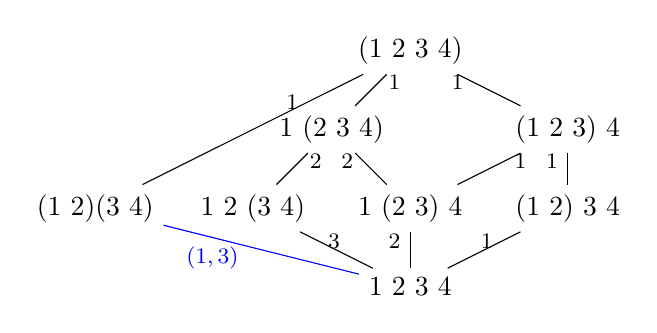
\begin{tikzpicture}[rotate =180 ]
				%Noeud du diagramme
				\node (P0) at (0,0) {$(1~2~3~4)$};
				\node (P11) at (-2,1) {$(1~2~3)~4$};
				\node (P12) at (4,2) {$(1~2)(3~4)$};
				\node (P13) at (1,1) {$1~(2~3~4)$};
				\node(P21) at (-2,2) {$(1~2)~3~4$};
				\node(P22) at (0,2) {$1~(2~3)~4$};
				\node(P23) at (2,2) {$1~2~(3~4)$};
				\node(P31) at (0,3) {$1~2~3~4$};
				%Arêtes du poset
				\draw (P0) -- (P11) node[left,near start] {\footnotesize{$1$}};
				\draw (P0) -- (P12) node[left,near start] {\footnotesize{$1$}};
				\draw (P0) -- (P13) node[right,near start] {\footnotesize{$1$}};
				\draw (P11) -- (P21) node[left,near start] {\footnotesize{$1$}};
				\draw (P11) -- (P22) node[right,near start] {\footnotesize{$1$}};
				\draw[blue] (P12) -- (P31) node[below,near start] {\footnotesize{$(1,3)$}};
				\draw (P13) -- (P22) node[left,near start] {\footnotesize{$2$}};
				\draw (P13) -- (P23) node[right,near start] {\footnotesize{$2$}};
				\draw (P22) -- (P31) node[left,near start] {\footnotesize{$2$}};
				\draw (P21) -- (P31) node[left,near start] {\footnotesize{$1$}};
				\draw (P23) -- (P31) node[right,near start] {\footnotesize{$3$}};
			\end{tikzpicture}
	\end{figure}

Note that in this poset, a Shroeder tree with 4 leaves is exactly an initial chain of this poset.

\begin{Eg}
	In the poset of figure~\ref{fig:IP4}, the two following initial chains gives the same tree:
	\begin{align*}
		1~2~3~4 \leq 1~2~(3~4) &\leq (1~2)(3~4) \leq (1~2~3~4), \\
		1~2~3~4 \leq (1~2)~3~4 &\leq (1~2)(3~4) \leq (1~2~3~4)
	\end{align*}
	Meanwhile, in the modified poset of figure~\ref{fig:tree4_poset}, this tree is represented by the unique initial chain:
	\[
	1~2~3~4 \leq (1~2)(3~4) \leq (1~2~3~4).
	\]
\end{Eg}
\begin{Rq}
	Note that the number of initial chains in the poset of figure~\ref{fig:IP4} is:
	\[
	1+6+6=13,
	\]  whereas the number of initial chains in the modified poset of figure~\ref{fig:tree4_poset} is:
	\[
	1+6+4=11
	\]
	the $4$-th Schroeder number.
\end{Rq}

For more details let us consider the $\IP{5}$ poset in figure~\ref{fig:IP5}:
\begin{figure}
	\label{fig:IP5_whole}
	\centering
	\caption{The construction on $\IP{5}$}
	\begin{subfigure}{0.9\textwidth}
	\label{fig:IP5}
	\centering
	\subcaption{The 5-tree poset}	
	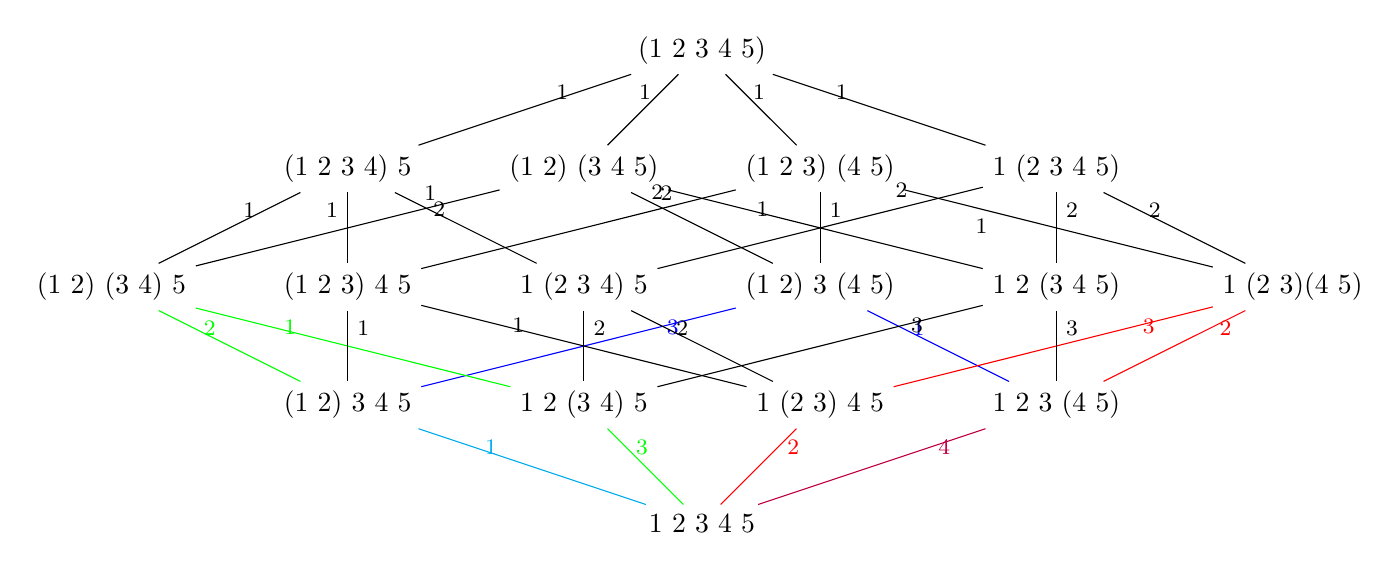
\begin{tikzpicture}[rotate=180, x=1.5cm, y=1.5cm]
		%Noeud du diagramme, le noeud du noeud est donné par la suite des tailles des blocs
		\node (P5) at (0,0) {$(1~2~3~4~5)$};
		\node (P14) at (-3,1) {$1~(2~3~4~5)$};
		\node(P23) at (1,1) {$(1~2)~(3~4~5)$};
		\node(P32) at (-1,1) {$(1~2~3)~(4~5)$};
		\node(P41) at (3,1) {$(1~2~3~4)~5$};
		
		\node (P122) at (-5,2) {$1~(2~3)(4~5)$};
		\node (P311) at (3,2) {$(1~2~3)~4~5$};
		\node(P212) at (-1,2) {$(1~2)~3~(4~5)$};
		\node(P131) at (1,2) {$1~(2~3~4)~5$};
		\node(P113) at (-3,2) {$1~2~(3~4~5)$};
		\node(P221) at (5,2) {$(1~2)~(3~4)~5$};
		
		\node (P1112) at (-3,3) {$1~2~3~(4~5)$};
		\node (P1211) at (-1,3) {$1~(2~3)~4~5$};
		\node (P1121) at (1,3) {$1~2~(3~4)~5$};
		\node (P2111) at (3,3) {$(1~2)~3~4~5$};
		
		\node (P11111) at (0,4) {$1~2~3~4~5$};
		%Arêtes du poset
		\draw (P5) -- (P14) node[right,near start] {\footnotesize{$1$}};
		\draw (P5) -- (P41) node[left,near start] {\footnotesize{$1$}};
		\draw (P5) -- (P32) node[right,near start] {\footnotesize{$1$}};
		\draw (P5) -- (P23) node[left,near start] {\footnotesize{$1$}};
		
		\draw (P32) -- (P212) node[right,near start] {\footnotesize{$1$}};
		\draw (P32) -- (P122) node[below,near start] {\footnotesize{$1$}};
		\draw (P32) -- (P311) node[above,near start] {\footnotesize{$2$}};
		\draw (P14) -- (P122) node[right,near start] {\footnotesize{$2$}};
		\draw (P14) -- (P113) node[right,near start] {\footnotesize{$2$}};
		\draw (P14) -- (P131) node[above,near start] {\footnotesize{$2$}};
		\draw (P41) -- (P131) node[above,near start] {\footnotesize{$1$}};
		\draw (P41) -- (P221) node[left,near start] {\footnotesize{$1$}};
		\draw (P41) -- (P311) node[left,near start] {\footnotesize{$1$}};
		\draw (P23) -- (P212) node[above,near start] {\footnotesize{$2$}};
		\draw (P23) -- (P113) node[right,near start] {\footnotesize{$1$}};
		\draw (P23) -- (P221) node[right,near start] {\footnotesize{$2$}};
		
		\draw[blue] (P212)--(P1112) node[right,near start]{\footnotesize{$1$}};
		\draw[blue] (P212)--(P2111) node[right,near start]{\footnotesize{$3$}};
		\draw[red] (P122)--(P1112) node[right,near start]{\footnotesize{$2$}};
		\draw[red] (P122)--(P1211) node[right,near start]{\footnotesize{$3$}};
		\draw (P131)--(P1211) node[right,near start]{\footnotesize{$2$}};
		\draw (P131)--(P1121) node[right,near start]{\footnotesize{$2$}};
		\draw (P113)--(P1121) node[right,near start]{\footnotesize{$3$}};
		\draw (P113)--(P1112) node[right,near start]{\footnotesize{$3$}};
		\draw[green] (P221)--(P1121) node[right,near start]{\footnotesize{$1$}};
		\draw[green] (P221)--(P2111) node[right,near start]{\footnotesize{$2$}};
		\draw (P311)--(P2111) node[right,near start]{\footnotesize{$1$}};
		\draw (P311)--(P1211) node[right,near start]{\footnotesize{$1$}};
		
		\draw[cyan] (P2111)--(P11111) node[right,near start]{\footnotesize{$1$}};
		\draw[red] (P1211)--(P11111) node[right,near start]{\footnotesize{$2$}};
		\draw[green] (P1121)--(P11111) node[right,near start]{\footnotesize{$3$}};
		\draw[purple] (P1112)--(P11111) node[right,near start]{\footnotesize{$4$}};
	\end{tikzpicture}
	\end{subfigure}
	\begin{subfigure}{0.9\textwidth}
		\centering
		\label{fig:simplifications}
		\caption{Simplifying the first row is enough}
		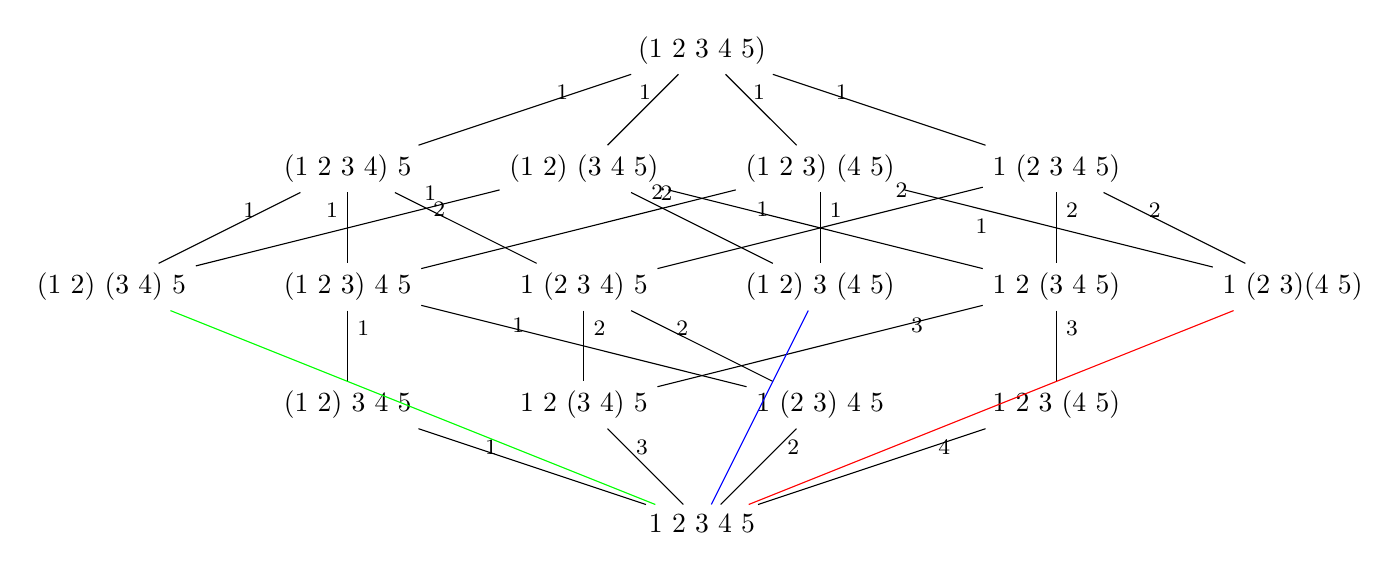
\begin{tikzpicture}[rotate=180, x=1.5cm, y=1.5cm]
			%Noeud du diagramme, le noeud du noeud est donné par la suite des tailles des blocs
			\node (P5) at (0,0) {$(1~2~3~4~5)$};
			\node (P14) at (-3,1) {$1~(2~3~4~5)$};
			\node(P23) at (1,1) {$(1~2)~(3~4~5)$};
			\node(P32) at (-1,1) {$(1~2~3)~(4~5)$};
			\node(P41) at (3,1) {$(1~2~3~4)~5$};
			
			\node (P122) at (-5,2) {$1~(2~3)(4~5)$};
			\node (P311) at (3,2) {$(1~2~3)~4~5$};
			\node(P212) at (-1,2) {$(1~2)~3~(4~5)$};
			\node(P131) at (1,2) {$1~(2~3~4)~5$};
			\node(P113) at (-3,2) {$1~2~(3~4~5)$};
			\node(P221) at (5,2) {$(1~2)~(3~4)~5$};
			
			\node (P1112) at (-3,3) {$1~2~3~(4~5)$};
			\node (P1211) at (-1,3) {$1~(2~3)~4~5$};
			\node (P1121) at (1,3) {$1~2~(3~4)~5$};
			\node (P2111) at (3,3) {$(1~2)~3~4~5$};
			
			\node (P11111) at (0,4) {$1~2~3~4~5$};
			%Arêtes du poset
			\draw (P5) -- (P14) node[right,near start] {\footnotesize{$1$}};
			\draw (P5) -- (P41) node[left,near start] {\footnotesize{$1$}};
			\draw (P5) -- (P32) node[right,near start] {\footnotesize{$1$}};
			\draw (P5) -- (P23) node[left,near start] {\footnotesize{$1$}};
			
			\draw (P32) -- (P212) node[right,near start] {\footnotesize{$1$}};
			\draw (P32) -- (P122) node[below,near start] {\footnotesize{$1$}};
			\draw (P32) -- (P311) node[above,near start] {\footnotesize{$2$}};
			\draw (P14) -- (P122) node[right,near start] {\footnotesize{$2$}};
			\draw (P14) -- (P113) node[right,near start] {\footnotesize{$2$}};
			\draw (P14) -- (P131) node[above,near start] {\footnotesize{$2$}};
			\draw (P41) -- (P131) node[above,near start] {\footnotesize{$1$}};
			\draw (P41) -- (P221) node[left,near start] {\footnotesize{$1$}};
			\draw (P41) -- (P311) node[left,near start] {\footnotesize{$1$}};
			\draw (P23) -- (P212) node[above,near start] {\footnotesize{$2$}};
			\draw (P23) -- (P113) node[right,near start] {\footnotesize{$1$}};
			\draw (P23) -- (P221) node[right,near start] {\footnotesize{$2$}};
			
			\draw (P131)--(P1211) node[right,near start]{\footnotesize{$2$}};
			\draw (P131)--(P1121) node[right,near start]{\footnotesize{$2$}};
			\draw (P113)--(P1121) node[right,near start]{\footnotesize{$3$}};
			\draw (P113)--(P1112) node[right,near start]{\footnotesize{$3$}};
			\draw (P311)--(P2111) node[right,near start]{\footnotesize{$1$}};
			\draw (P311)--(P1211) node[right,near start]{\footnotesize{$1$}};
			
			\draw (P2111)--(P11111) node[right,near start]{\footnotesize{$1$}};
			\draw (P1211)--(P11111) node[right,near start]{\footnotesize{$2$}};
			\draw (P1121)--(P11111) node[right,near start]{\footnotesize{$3$}};
			\draw (P1112)--(P11111) node[right,near start]{\footnotesize{$4$}};
			
			%Nouvelles arêtes
			\draw[red] (P122)--(P11111);
			\draw[green] (P221)--(P11111);
			\draw[blue] (P212)--(P11111);
		\end{tikzpicture}
	\end{subfigure}
\end{figure}

After applying the rule on the first raw, one gets the figure~\ref{fig:simplifications}.

This property of simplification in a poset needs more than just a poset. We need a map $\pi:P\times P \rightarrow \{0,1\}$ that tells us whether we can perform a "parallelisation simplification rule", for instance consider the subposet of the poset $\IP{6}$ given in figure~\ref{fig:part_IP6}:
\begin{figure}
	\centering
	\label{fig:part_IP6}
	\caption{Example over IP6}
	\begin{subfigure}{0.5\textwidth}
		\label{fig:aprt_IP6}
		\caption{The subposet of IP6}
		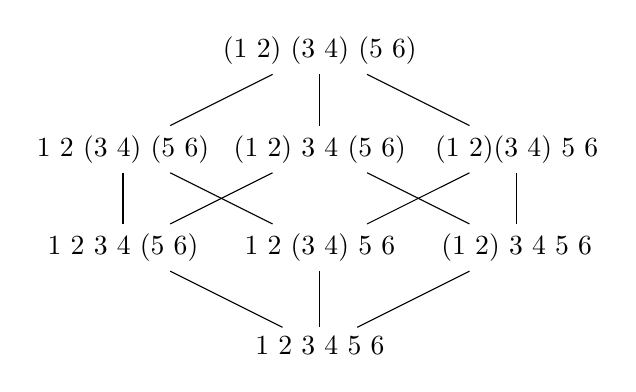
\begin{tikzpicture}[rotate=180, x=1.25cm, y=1.25cm]
		%Noeud du diagramme
		\node (P222) at (0,0) {$(1~2)~(3~4)~(5~6)$};
		\node (P2112) at (0,1) {$(1~2)~3~4~(5~6)$};
		\node (P2211) at (-2,1) {$(1~2)(3~4)~5~6$};
		\node (P1122) at (2,1) {$1~2~(3~4)~(5~6)$};
		\node(P21111) at (-2,2) {$(1~2)~3~4~5~6$};
		\node(P11211) at (0,2) {$1~2~(3~4)~5~6$};
		\node(P11112) at (2,2) {$1~2~3~4~(5~6)$};
		\node(P111111) at (0,3) {$1~2~3~4~5~6$};
		%Arêtes du poset
		\draw (P222) -- (P2112) node[left,near start] {};
		\draw (P222) -- (P2211) node[left,near start] {};
		\draw (P222) -- (P1122) node[right,near start] {};
		\draw (P2112) -- (P21111) node[left,near start] {};
		\draw (P2112) -- (P11112) node[right,near start] {};
		\draw (P2211) -- (P11211) node[below,near start] {};
		\draw (P2211) -- (P21111) node[left,near start] {};
		\draw (P1122) -- (P11211) node[right,near start] {};
		\draw (P1122) -- (P11112) node[left,near start] {};
		\draw (P21111) -- (P111111) node[left,near start] {};
		\draw (P11211) -- (P111111) node[right,near start] {};
		\draw (P11112) -- (P111111) node[right,near start] {};
		\end{tikzpicture}
	\end{subfigure}
	
	\begin{subfigure}{0.5\textwidth}
		\label{fig:first-row_IP6}
		\caption{Simplification of the first row}
		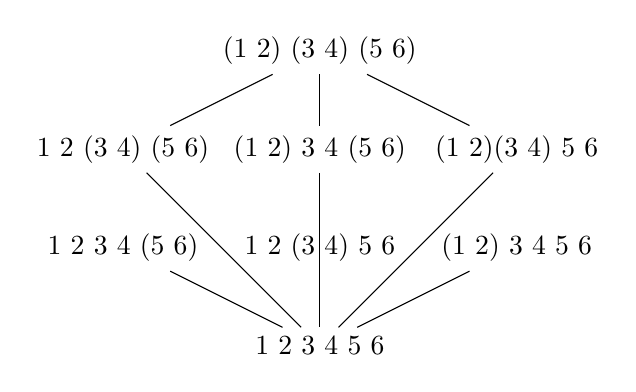
\begin{tikzpicture}[rotate=180, x=1.25cm, y=1.25cm]
			%Noeud du diagramme
			\node (P222) at (0,0) {$(1~2)~(3~4)~(5~6)$};
			\node (P2112) at (0,1) {$(1~2)~3~4~(5~6)$};
			\node (P2211) at (-2,1) {$(1~2)(3~4)~5~6$};
			\node (P1122) at (2,1) {$1~2~(3~4)~(5~6)$};
			\node(P21111) at (-2,2) {$(1~2)~3~4~5~6$};
			\node(P11211) at (0,2) {$1~2~(3~4)~5~6$};
			\node(P11112) at (2,2) {$1~2~3~4~(5~6)$};
			\node(P111111) at (0,3) {$1~2~3~4~5~6$};
			%Arêtes du poset
			\draw (P222) -- (P2112) node[left,near start] {};
			\draw (P222) -- (P2211) node[left,near start] {};
			\draw (P222) -- (P1122) node[right,near start] {};
			
			\draw (P2112) -- (P111111) node[left,near start] {};
			\draw (P2211) -- (P111111) node[below,near start] {};
			\draw (P1122) -- (P111111) node[right,near start] {};
			
			\draw (P21111) -- (P111111) node[left,near start] {};
			\draw (P11211) -- (P111111) node[right,near start] {};
			\draw (P11112) -- (P111111) node[right,near start] {};
		\end{tikzpicture}
	\end{subfigure}
	
	\begin{subfigure}{0.5\textwidth}
		\label{fig:second-row_IP6}
		\caption{Simplification of the second row}
		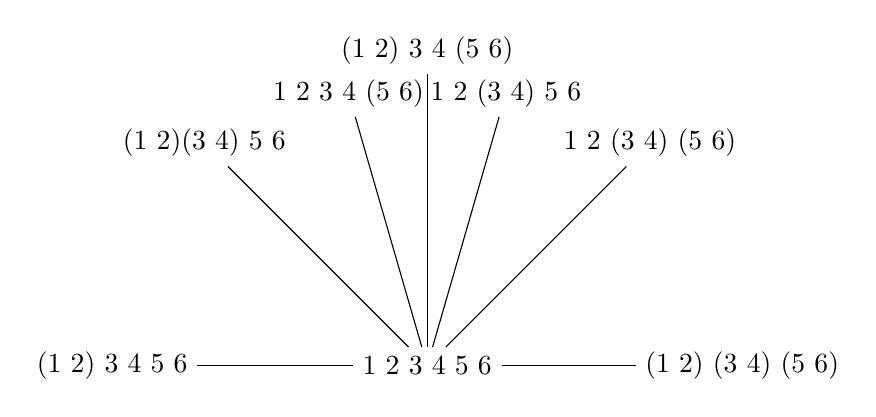
\begin{tikzpicture}[ x=1cm, y=1cm]
			%Noeud du diagramme
			\node (P222) at (4,0) {$(1~2)~(3~4)~(5~6)$};
			\node (P2112) at (0,4) {$(1~2)~3~4~(5~6)$};
			\node (P2211) at (-2.83,2.83) {$(1~2)(3~4)~5~6$};
			\node (P1122) at (2.83,2.83) {$1~2~(3~4)~(5~6)$};
			\node(P21111) at (-4,0) {$(1~2)~3~4~5~6$};
			\node(P11211) at (1,3.46) {$1~2~(3~4)~5~6$};
			\node(P11112) at (-1,3.46) {$1~2~3~4~(5~6)$};
			\node(P111111) at (0,0) {$1~2~3~4~5~6$};
			%Arêtes du poset
			\draw (P222) -- (P111111) node[left,near start] {};
			\draw (P11211) -- (P111111) node[left,near start] {};
			\draw (P11112) -- (P111111) node[right,near start] {};
			\draw (P21111) -- (P111111) node[right,near start] {};
			\draw (P2112) -- (P111111) node[left,near start] {};
			\draw (P2211) -- (P111111) node[below,near start] {};
			\draw (P1122) -- (P111111) node[right,near start] {};
		\end{tikzpicture}
		\end{subfigure}
\end{figure}